\documentclass[11pt, oneside]{article}
\usepackage{latexrc}
\usepackage{hyperref}
\usepackage{float}

\title{CS3110 Hnefatafl Design Doc}
\author{Elizabeth VanDenburgh (eav38)\and Joseph Dwyer (jmd456)\and Taeer Bar-Yam (tb442)}
\date{November, 12 2015}

\begin{document}

\maketitle

\section{Structure of the Implementation}
The Hnefatafl game that we created is a historic Viking game with several different play modes.
The board game was created by the Vikings and is meant to simulate the defense and attack
of two uneven sides.  The defenders goal is to protect their king and move the king to specific
locations on the board.  The attacks want to capture the king.  Because this is a historic
game, there are several different versions (we call them modes).
The modes differ in their rule sets and initial configurations.
They are each described in detail below. To increase the complexity of the game, we implemented
TWO/THREE different game modes.  We allow the player
to decide, at runtime, what version on the game they would like to play.  The rules
and intial setup of the game are then loaded into the main program and the player
can begin.

\section{Hnefatafl Game Mode Descriptions}
\subsection{CS3110 Hnefatafl}
We created this version of the game after our inital study of the rules.  After further study
we realized that this game mode is not as accurate historically as Fetlar.  For this reason, we
are leaving this mode of the game as the default (because it is the easiest to explain and understand)
but naming it CS3110 Hnefatafl (because it does not perfectly match any true rule set).\\
The game is played on an $9\times 9$ checkered board with two uneven sides.
$8$ white pieces are positioned around a white ``king'' at the center of the
board creating a cross, with $16$ black pieces arranged on the edges surrounding them.

The black team moves first.

There are three main mechanics involved in the game:
\begin{enumerate}
\item \textbf{Movement}\\
  Pieces move like rooks in chess (horizontally or vertically).
  Only the king has a limited motion of three squares at a time.
\item \textbf{Capturing}\\
  When a piece is flanked by two pieces of the opposing color, that piece is
  ``captured'' and is removed from the board.  This flanking must be done
  actively by the offense (i.e. the center piece can move between the others
  without being captured).\\
  The king cannot participate in flanking an opponent. In the case of the king,
  it must be flanked on all sides to be considered ``captured.''
\item \textbf{Winning}\\
  Black wins when the king is captured.\\
  White wins when the king is moved to one of the side squares of the board.
\end{enumerate}
See: \url{https://en.wikipedia.org/wiki/Tafl\_games\#Hnefatafl}

\subsection{Fetlar Hnefatafl}
This is a true version of the game.  The setup is an $11\times11$ checkered board with $12$ white
pieces positioned around the white ``king'' at the center and $24$ black pieces around the edges of the board. The black team moves first.

See~\ref{fig:initial_position}.
\begin{figure}\label{fig:initial_position}
  \centering
  \scalebox{.5}{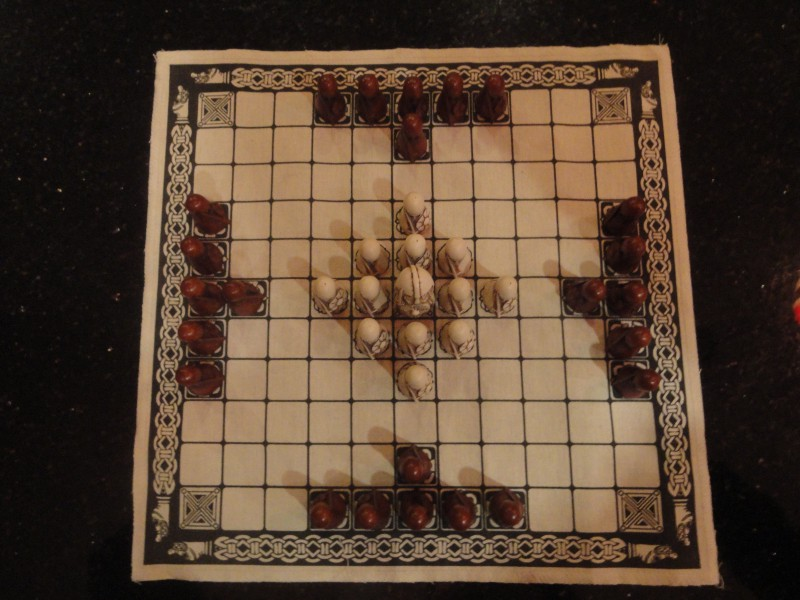
\includegraphics{hnefatafl}}
  \caption{Hnefatafl starting board position. Source: \url{https://medium.com/war-is-boring/you-have-to-play-this-1-600-year-old-viking-war-game-cef088ae4e2d\#.10kof827g}}
\end{figure}

Main mechanics of Fetlar:
\begin{enumerate}
\item \textbf{Restricted Squares}\\
  In this version of the game, there are restricted squares.  These are the throne (center square of the board) and the four corner squares.  These squares limit the movement of pawns and can be involved in captures.
\item \textbf{Movement}\\
  Pieces move like rooks in chess (horizontally or vertically).
  There is no limit on the number of pieces that the king can move.
  Pawns cannot land on a restricted square.  They can, however, pass through the throne if it is unoccupied by the white king.
\item \textbf{Capturing}\\
  Capturing in Fetlar is very similar to capturing in our default game.  Capturing of pawns is done by actively flanking them (sandwiching the captured piece between two opponents).  Capturing of the king is done by actively flanking him by surrounding him on all four sides.  In this version, however, the king can participate in captures.  There are also the restricted squares.  This means that the 5 restricted squares can replace one of the attacking pieces in a flanking move.  Even with the restricted squares, black cannot capture the king when he is against a wall.  The throne square will always be hostile to black pieces and it will be hostile to white pieces when it is empty. This means that the king can be captured if he sits immediately next to the throne and is surrounded on the other 3 sides by black pieces.
\item \textbf{Winning}\\
  The black team wins by capturing the king.  The white team wins by having the king escape.  He does this by landing on a corner square.
\end{enumerate}

\subsection{Copenhagan Hnefatafl}
This is a harder form of Hnefatafl, but it has similar features to Fetlar.  The thing that makes this game more difficult is additional ways that pieces can be captured.

Main mechanics of Copenhagan:
\begin{enumerate}
\item \textbf{Restricted Squares}\\
  This is the same idea as Fetlar.
\item \textbf{Movement}\\
  The same rules apply as in Fetlar.
\item \textbf{Capturing}
  The generics of capturing are the same as Fetlar. There is an additional way of capturing called a shieldwall.  This is accomplished by bracketing the opposing team against a wall.  For this move to be complete, the offensive team must be placed one in front of each defensive player, backing them into a wall.  The line of defensive pieces must also be pegged in on the bookends with an offensive piece. A corner square can also act as a bookend piece. You can capture as many pieces as you want by doing this move.  This includes capture of the king.
\item \textbf{Winning}
  Once again, the king must move to the corner squares to escape.  White wins when this occurs.  The black team wins when the king is captured.
\end{enumerate}


\section{Interface:}
There are three possible GUIs that the user can decide between at runtime.  They include a text-based interface, a 2D interface, and a 3D interface.  They are described below.  Every GUI includes the command that q and esc are quit.  This means quitting up to a higher level menu. If you quit a game, there is no way to re-enter it.  It is important to use the q and esc keys when quitting a GUI because they are pre-programmed to exit gracefully.  Users that do not use these keys will see errors in their terminal.

\subsection{Text-Based}
We call this GUI "ascii".  It is in the file named "ascii.ml".  The controls for this GUI are the arrow buttons (or hjkl) to move.  The space bar selects a piece.  The location of the cursor is shown with a blue, highlighted square.  This GUI is implemented using Termbox which takes over the terminal that called the function.

\subsection{2-Dimensional}
We call this GUI "2D".  It is in the file named "graphical.ml".  The controls for this GUI are clicking and dragging with the mouse.  A selected piece moves with the mouse.  This GUI is implemented using the built-in OCaml graphics library.  It opens a new window.

\subsection{3-Dimensional}
We call this GUI "3D". It is in the file named "threeD.ml".  The controls for this GUI are arrow keys (and hjkl).  The cursor is shown with a lit tile.  Selection of a piece is done with the space bar.  This GUI is implemented using OpenGL and it opens a new window.

\section{Artificial Intelligence}
The AI computes, with no data structure, the optimal move at each turn.  The optimal move is computed using a utility function.  The utility function is dependent on the number of captured pieces and the distance of the white king to the win condition.  White and black actually use the same utility function.  This helps the black team not only capture pieces, but oppose the movement of the white king.  Relating the number of pieces captured to the movement of the king was one design consideration.  If you value the kings movement too highly, the white team AI will rush to the win condition with little consideration for the welfare of its pieces.  If you value the movement too little, the white AI turtles and only defends that king without actively trying to win.  We determined the valuation ratio between a lost piece and movement of the king by having AI with randomly generated constants play against each other and take the best value.  This is an informal version of a neural-network.

\section{Menus}

\section{Architecture}
\begin{figure}[H]\label{fig:CCD}
  \centering
  \scalebox{0.5}{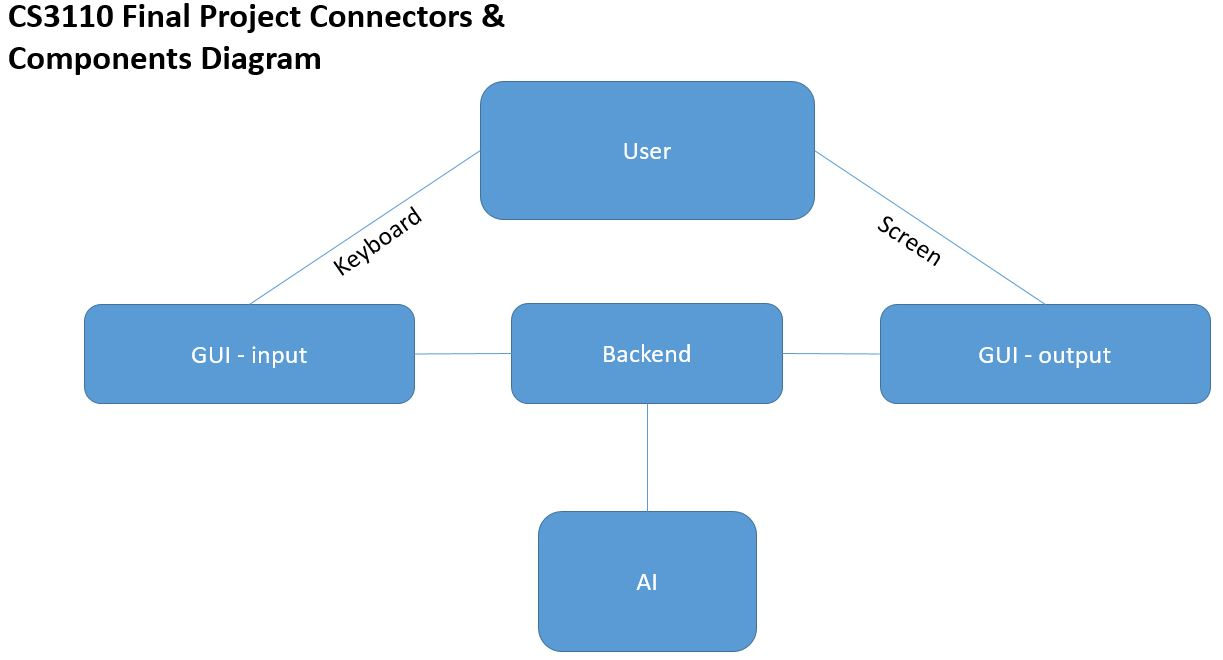
\includegraphics{CCD}}
  \caption{Connector Component Diagram of the pipe and filter architecture for
    our project. Unmarked lines represent connections via function calls
    (APIs).}
\end{figure}
The backend forms a pipe-and-filter architecture that applies an attempted move
to the board state given the rules of the game. The backend and AI components
form a server-client like connection where the backend communicates with the AI
code to determine what the best move is. In this case the AI is the server and
the backend is the client. See~\ref{fig:CCD} for the connector and component
diagram.

\section{System Design}
\begin{figure}[H]\label{fig:MDD}
  \centering
  \scalebox{0.5}{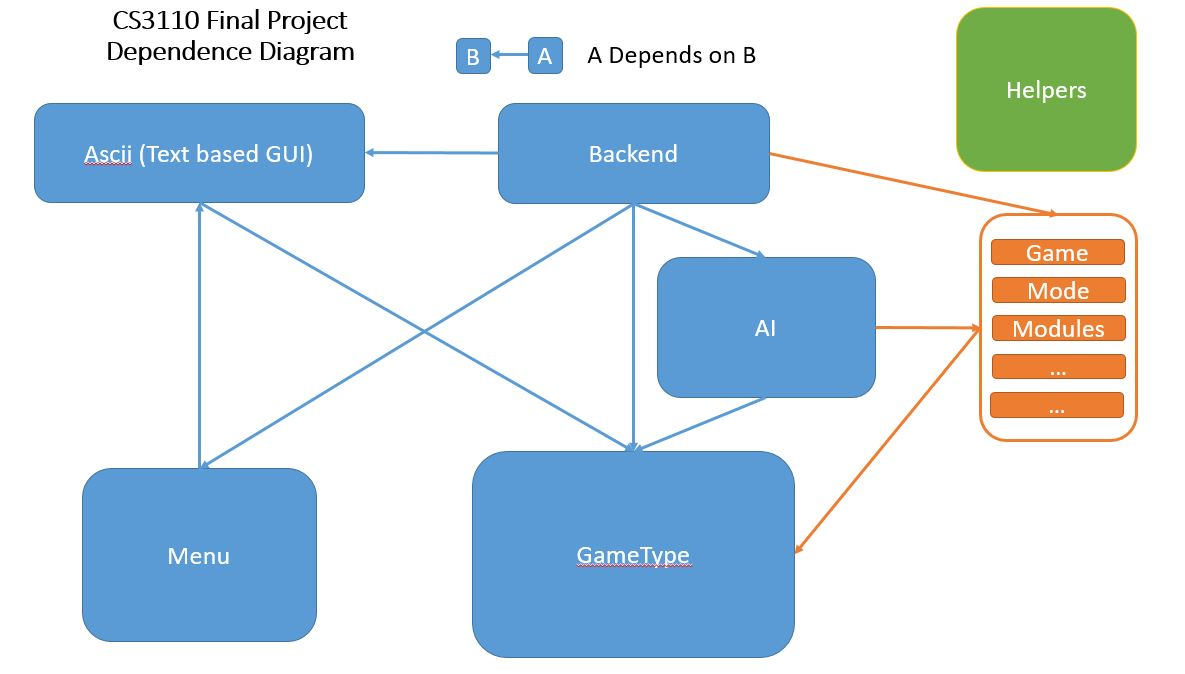
\includegraphics{MDD}}
  \caption{Diagram of dependencies between modules in our project. The helpers
    module (green) is depended on by everything. The game mode modules (orange)
    may or may not end up in the final version}
\end{figure}

\subsection{GUI}
Two options of GUI modules: Text-based and graphical.\\
The purpose of this module is to enable interaction between the user and the
backend. The GUI does none of the game or board computations. It only has
knowledge of the screen state, and what the backend tells it to print. It
\textbf{is} in charge of interpreting piece movement by the user. That is, it
does not report every keystroke, mouseclick, etc. the user makes, only what move
the user would like to make.

\subsection{Main}
Main is in charge of the following tasks:
\begin{itemize}
\item Initialization of menu and storage of configuration options
\item Keeps track of the baord and player state
\item Validates moves from the GUI
\item Calculates if a move resulted in a piece's capture
\item Calculates if the game is over and who won
\item Calculates if the game is unwinable (hopefully)
\item Prompts the GUI for the user's next move
\item Prompts the AI for it's next move
\end{itemize}

\subsection{Menu}
In the Menu module is what text to display in the start of game menus. It tells
the GUI which menus to display and the GUI responds with which selection the
user made. The menu composes a game configuration based on the choices and
passes that back to the Backend.\\
Menu will also present a ``Do you want to quit?'' type message on quit.

\subsection{AI}
If playing as one person, the AI module will be passed the current board state
by the Backend. Using this, it will create a decision tree and decide on an
``intelligent'' move
to execute.\\
We can put the AI calls in a separate thread to allow more computation for a
smarter AI.\\\\
Ideally we would like to create either a general AI for all game modes or a
stronger AI for each individual game mode. Based on the amount of time that we
have, and the complexity of building such AI, we will decide which AI
implementation to use.

\subsection{Helpers}
Basic functions that either we feel should have been included in OCaml or most
modules will need are included in Helpers.

\subsection{GameType}
GameType includes basic types for the board, pieces on the board, and other
game-state related objects. It also includes small helper functions that relate
to those types. (e.g. piece\_at for the piece at a location on the board)

\subsection{GameModes?}
We have two ideas for how to implement variants on the game mode (e.g.
differences in win conditions, valid movements, etc.). One involves dynamically
loading one of a set of module that will contain functions for these aspects of
the game.\\
The alternative would be to load preferences out of a plain text file.\\\\
\textit{Pros/Cons:}
\begin{description}
\item[+] Doesn't require us to write text parsing code
\item[+] More flexible (can run arbitrary code)
\item[-] Less secure (can run arbitrary code)
\item[-] Dynamically loading modules is awkward
\end{description}

\section{Module Design}
See attached .mli files.

\section{Data}
Structures include:
\begin{itemize}
\item Piece types (variant)
\item Coordinates (type synonym for int * int)
\item Action variant (what actions the user can perform)
\item Game configurations
\item Board with dimensions and list of piece locations
\end{itemize}

State data:
\begin{itemize}
\item Which player's turn it is
\item Current board state
\item Which game configuration was selected
\end{itemize}
The GUI also stores the current selected piece (the piece the user would like to
move) until the user selects a location to move it to.

Everything is passed through function calls. There is no imperative or global
data.

\section{External Libraries}
\begin{itemize}
\item Termbox for creating an ascii board
\item OpenGL for creating a more graphical gui
\item Potentially Dynlink for dynamically linking game modes
\end{itemize}

\section{Testing Plan}
\begin{itemize}
\item Write unit tests for state of the board after certain moves
  \begin{itemize}
  \item Valid moves
  \item Invalid moves
  \item Win conditions
  \item Piece removal conditions
  \item All of these, in various game modes
  \end{itemize}
\item Watch the AI play against itself
\item Get play testers
\end{itemize}

\section{Division of Labor}
\begin{itemize}
\item Joseph
\item Taeer
  \begin{itemize}
  \item Fetlar.ml
    \begin{itemize}
    \item Initial board setup
    \end{itemize}
  \end{itemize}
\item Elizabeth
  \begin{itemize}
  \item Prepared final Design Document
  \item Default.ml
    \begin{itemize}
    \item Winning conditions
    \item Capturing pieces
    \item Initial board setup
    \end{itemize}
  \item Fetlar.ml
    \begin{itemize}
    \item Winning conditions
    \item Capturing pieces
    \end{itemize}
  \item Copenhagan.ml
    \begin{itemize}
    \item Winning conditions
    \item Capturing pieces
    \end{itemize}
  \end{itemize}
\end{itemize}

\end{document}
